\newpage
\section{Basic Topology}
\subsection{Finite and Countable Sets}
This chapter is split into two portions; the first looks at counting, what it means for us to say that two sets have the same number of elements, and concludes with a classic theorem of Cantor concerning uncountable sets. The second part looks at the topology of metric spaces, before moving onto the topology of the real numbers. 

Let us then begin with our discussion of counting. If we consider counting how many bananas there are on a table (say there are 10 bananas), then what we are formally doing is establishing a correspondence between each ball on the table with an element in the set $\set{1, \ldots, 10}$. When we refer to the number of elements in a set, it will be good to keep in mind that we are establishing functions between sets. Although we have been discussing functions with some frequency in the course already, we give a definition below for completeness. 

\begin{definition}{Functions}{2.1}
    Let $A, B$ be sets. Then, a map that associates each element $x \in A$ with a unique element denoted as $f(x) \in B$ is a \textbf{function} $f: A \rightarrow B$. We then define $A$ as the \textbf{domain} of $f$ and the set $\set{f(x): x \in A}$ as the \textbf{range}. For $E \subseteq A$, we call $f(E) = \set{f(x): x \in E}$ the \textbf{image} of $E$ under $f$. For $F \subseteq B$, we call $f^{-1}(B) = \set{x \in A: f(x) \in B}$ the \textbf{preimage} of $F$. 
\end{definition}

\begin{definition}{Injective/Surjective Functions}{2.2}
    Let $f: A \mapsto B$ be a function. If for $x_1, x_2 \in A$ we have that $f(x_1) = f(x_2) \implies x_1 = x_2$ (or equivalently, $x_1 \neq x_2 \implies f(x_1) \neq f(x_2)$), then we say that $f$ is \textbf{injective}, or \textbf{one-to-one}. If for all $y \in B$ there exists $x \in A$ such that $y = f(x)$, then we say that $f$ is \textbf{surjective}, or \textbf{onto}. If a function is both injective and surjective, it is \textbf{bijective}.
\end{definition}
\noindent Intuitively, we can think of injectivity as implying each element in $B$ being reached at most once, and surjectivity implying that each element in $B$ is reached at least once. 

\begin{definition}{Cardinality \& Equivalence}{2.3}
    Let $A, B$ be sets. We say that $A, B$ have the same \textbf{cardinality} if there exists $f: A \mapsto B$ such that $f$ is bijective. We can denote this as $A \sim B$ where $\sim$ indicates an \textbf{equivalence relation}. An equivalence relation has three properties:
    \begin{enumerate}
        \item Reflexivity: $A \sim A$.
        \item Symmetry: If $A \sim B$ then $B \sim A$.
        \item Transitivity: If $A \sim B$ and $B \sim C$ then $A \sim C$.
    \end{enumerate}
    As a point of notation, $\abs{S}$ denotes the cardinality of the set $S$. 
\end{definition}

\noindent We get (a) from each set having a bijection to itself (i.e. the identity function), (b) from the fact that if there exists a bijection $f: A \mapsto B$, then there must exist an inverse $f^{-1}: B \mapsto A$, and (c) from if there exist bijections $f: A \mapsto B$ and $g: B \mapsto C$ then the composition $g \circ f: A \mapsto C$ will also be a bijection. 

\begin{definition}{Countability}{2.4}
    First, we denote $J_n = \set{1, 2, 3, \ldots, n}$ and $J = \NN = \set{1, 2, 3, \ldots}$. Let $A$ be a set. We say that $A$ is \textbf{finite} if it has a finite number of elements, that is, there exists $n \in \NN$ such that $A \sim J_n$. A set $A$ is \textbf{infinite} if it is not finite, and we cannot put $A$ in bijection with $J_n$ for any $n \in \NN$. We say that $A$ is \textbf{countable}if $A \sim \NN$, and \textbf{uncountable} otherwise. 
\end{definition}

\noindent Note that the above definition gives us a useful notion for what sets we can consider countable; if we can enumerate a set with the naturals, this yields a bijection with $\NN$ and hence the set must be countable. 

We here give some additional properties concerning cardinalities of sets, which may be useful:
\begin{itemize}
    \item $\abs{A} \leq \abs{B} \iff \exists f: A \mapsto B \text{ such that $f$ is injective}$
    \item $\abs{A} \geq \abs{B} \iff \exists f: A \mapsto B \text{ such that $f$ is surjective}$
    \item $\abs{A} \leq \abs{B} \text{ and } \abs{A} \geq \abs{B} \implies \abs{A} = \abs{B}$
\end{itemize}

\begin{example}{}{2.5}
    $\ZZ$ is countable. To see this, consider the function:
    \begin{align*}
        f = \begin{cases}
            \frac{n}{2} & \text{$n$ is even}
            \\ -\frac{n-1}{2} & \text{$n$ is odd}
            \end{cases}
    \end{align*}
    $f$ is a bijection (check!) and hence $\NN \sim \ZZ$. 
\end{example}
\noindent The above example serves as a bit of a warning sign. Even though $\NN \subsetneq \ZZ$ and $\ZZ$ has ``more elements'', we still find that the two sets have the same cardinality. A similar example is given by $\NN$ and the set of all even natural numbers (which we may denote $2\NN$); the bijection $f(n): n \mapsto 2n$ between these two sets shows that $\NN \sim 2\NN$, even though $2\NN$ is a strict subset of $\NN$. 
\setcounter{rudin}{7}

\begin{theorem}{}{2.8}
    A subset of a countable set is either finite or countable.
\end{theorem}
\begin{nproof}
    (Sketch) The countability of $A$ implies that $A = \set{a_1, a_2, a_3, a_4, a_5 \ldots}$ (in other words, we can enumerate the elements using $\NN$). Let $S \subseteq A$. Then, $S = \set{a_1, \cancel{a_2}, a_3, a_4, \cancel{a_5}, \ldots}$, that is, $A$ with some (or none) of the elements removed. Now, we can rename all the elements with $a_1, a_2, \ldots$; what we have left is again an enumeration, so it is yet again (at most) countable.
\end{nproof}
\noindent One potentially useful fact is that if we have a set $S$ and a function $f: \NN \mapsto S$ such that $f$ is surjective, then $S$ is at most countable. 

\begin{proof}
    Let $T = \set{n \in \NN: f(n) \neq f(m), \forall m = 1, 2, \ldots, m}$. We restrict $f: T \mapsto S$, then $f$ is injective by constructive. It is still surjective, hence $T \sim S$. Since $T \subset \NN$, by Theorem \ref{thm:2.8}, $S$ is finite or countable.
\end{proof}

\setcounter{rudin}{11}

\begin{theorem}{}{2.12}
    Let $E_1, E_2, \ldots$ be countable sets (i.e. we have a countable number of countable sets). Define $S = \bigcup_{n=1}^{\infty} E_n$. Then, $S$ is countable. 
\end{theorem}
\begin{nproof}
    Write $E_n = \set{x_{n1}, x_{n2}, x_{n3}, \ldots}$ (which we can do as each of the $E_n$s are countable). Then, we form an array:
    \begin{center}
    \begin{tikzpicture}
        \matrix[matrix of math nodes,inner sep=1pt,row sep=1em,column sep=1em] (M)
        {
            E_1 & = & x_{11} & x_{12} & x_{13}  & \cdots \\
            E_2 & = & x_{21} & x_{22} & x_{23}  & \cdots \\
            E_3 & = & x_{31} & x_{32} & x_{33}  & \cdots \\
            \cdots \\
        }
        ;
        \draw[->] (M-1-3.south west) -- (M-1-3.north east);
        \draw[->] (M-2-3.south west) -- (M-1-4.north east);
        \draw[->] (M-3-3.south west) -- (M-1-5.north east);
        \draw[->] (M-1-3.south west) -- (M-1-3.north east);
        \draw[->] (M-3-4.south west) -- (M-2-5.north east);
        \draw[->] (M-3-5.south west) -- (M-3-5.north east);
    \end{tikzpicture}
    \end{center}
    Then, we can re-number the elements along the diagonal lines (i.e. $x_{11}, x_{21}, x_{12}, x_{31}, x_{22}, x_{13}, \ldots$). This new enumeration corresponds to a countable set. From there, we let $T \subseteq \NN$ be the remaining labels in the enumeration after removing the repeated elements from the sequence. Then, $T \sim S$, and hence $S$ is at most countable. $S$ cannot be finite as $E_1 \subseteq S$ and $E_1$ is not finite. Hence $S$ is countable. \qed
\end{nproof}

\begin{corollary}{$\QQ$ is Countable.}{2.13}
    \begin{itemize}
        \item If $A$ is countable, the set of n-tuples of $(a_1, \ldots a_n)$ is also countable for any $n \in \NN$.  
        \item $\QQ$ is countable.
    \end{itemize}
\end{corollary}
\noindent We defined $\QQ$ as pairs of integers, but by the first part of the corollary (which follows immediately by application of Theorem \ref{thm:2.12}) $\ZZ^2$ (the set of pairs of integers) has equal cardinality to $\ZZ$, and since $\QQ$ is a subset of the set of pairs of integers, $\QQ$ is countable. 

From the discussion of today, we have established that $\abs{\NN} = \abs{\ZZ} = \abs{\QQ}$. Does $\RR$ also have equal cardinality to these sets? Do infinite sets in general have the same cardinality? The answer turns out to be no for both of these questions. We will answer the first question in the next lecture (when we discuss Cantor diagonalization, a highlight of the course), but we can discuss the second statement now. First, we make a definition:
\begin{ndef}{: Power Sets}
    Let $A$ be a set. Then, the \textbf{power set} of $A$, denoted $\mathcal{P}(A)$, is the set of all subsets of $A$. 
\end{ndef}
\noindent An interesting theorem then follows:
\begin{ntheorem}{: Power Set Cardinality}
    Let $A$ be a set. Then, $\abs{A} < \abs{\mathcal{P}(A)}$.
\end{ntheorem}
\begin{nproof}
    Suppose for the sake of contradiction that there exists a surjection $f: A\rightarrow \pset{A}$ (this would imply that $\abs{A} \geq \abs{\pset{A}}$, so by showing this is false, we obtain the desired result). Then, each element $x \in A$ gets mapped to some subset of $A$. We either have that $x$ belongs to the subset that it gets mapped to, or it doesn't. Therefore, we can define a new subset $B \subseteq A$, such that:
    \[B = \set{x\in A: x \notin f(x)}\]
    In other words, the set of all $x$s that are not in the subset that they get mapped to by $f$. Since $f$ is surjective, there must be an element $y \in A$ such that $f(y) = B$. One of $y \in B$, $y \notin B$ must be true. If $y \in B$, by construction of $B$ we have that $y$ is not in the subset that it gets mapped to by $f$, which is a contradiction. If $y \notin B$, by definition of $B$, $y \in B$ as it is not in the subset that it gets mapped to, yet again a contradiction. Therefore, we conclude that no $y \in A$ exists such that $f(y) = B$, and hence, no surjective $f$ exists such that $f: A \rightarrow \pset{A}$. Hence, $\abs{A} < \abs{\pset{A}}$. \qed
\end{nproof}
\noindent An interesting consequence of this theorem is that for a countable set $A$, we then have that $\mathcal{P}(A)$ is an infinite set which has greater cardinality! For example, $\abs{\NN} < \abs{\mathcal{P}(\NN)}$. Moreover, this gives rise to an infinite number of cardinalities in ascending order; $\abs{\NN} < \abs{\pset{\NN}} < \abs{\pset{\pset{\NN}}} < \cdots$ and so on.

\subsection{Uncountable Sets}
\begin{theorem}{Existence of Uncountable Sets}{2.14}
Let $A = \set{(b_1, b_2, \ldots), b_n \in \set{0, 1}}$ be the set of binary sequences. Then, $A$ is uncountable. 
\end{theorem}
\begin{nproof}
    It suffices to show that every countable subset of $A$ is a proper subset of $A$. Let $E \subset A$ be countable, and let $E = \set{S^{(1)}, S^{(2)}, S^{(3)}, \ldots}$. To show that $E$ is a proper subset, we show that there exists a sequence $S \in A \setminus E$. To construct such an $S$, let us put the elements of $E$ in an array. 
    \begin{center}
        \begin{tikzpicture}
            \matrix[matrix of math nodes,inner sep=1pt,row sep=1em,column sep=1em] (M)
            {
                S^{(1)} & = & \boxed{b_{1}^{1}} & b_{2}^{1} & b_{3}^{1} &  \cdots \\
                S^{(2)} & = & b_{1}^{2} & \boxed{b_{2}^{2}} & b_{3}^{2} & \cdots \\
                S^{(3)} & = & b_{1}^{3} & b_{2}^{3} & \boxed{b_{3}^{3}}  & \cdots \\
            };
        \end{tikzpicture}
    \end{center}
    Then, define:
    \[\tilde{b}_n^n = \begin{cases}
        1 & \text{if $b_n^n = 0$}
        \\ 0 & \text{if $b_n^n = 1$}
    \end{cases}\]
    I.e. $\tilde{b}_n^n$ is the bit flip of $b_n^n$. Then, let $S = (\tilde{b}_1^1, \tilde{b}_2^2, \tilde{b}_3^3, \ldots)$, that is, $S$ is the sequence of bit-flipped diagonal elements of the original array. By construction, $S \neq S^{(k)}$ as for any $S^{(k)} \in E$ as $S$ differs at the $k$th position. Hence, $S \notin E$ and therefore $E \subsetneq A$. \qed
\end{nproof}
\noindent The above proof is a very famous argument, invented by the mathematician George Cantor. The discovery that there exist sets with greater cardinality than $\NN$ was initially quite controversial in the math community!

\begin{ncorollary}{: $\RR$ is Uncountable}{}
    $\mathcal{P}(\NN)$ (the power set of $\NN$) is uncountable. $\RR$ is uncountable.
\end{ncorollary}
\begin{nproof}
    Although we showed that $\mathcal{P}(\NN)$ was uncountable last lecture, we show this in an alternative way by considering a bijection between $\mathcal{P}(\NN)$ and the set $A$ of binary sequences. To do this, consider that we can associate a subset $T \subset \NN$, $T \in \mathcal{P}(\NN)$ with the sequence corresponding to:
    \begin{align*}
        b_n = \begin{cases}
            1 & \text{if $n \in T$}
            \\ 0 & \text{if $n \notin T$}
        \end{cases}
    \end{align*}
    Since $A$ is uncountable, it follows that $\mathcal{P}(\NN)$ is uncountable. The second statement in the corollary follows (roughly) by considering $\RR$ represented in binary, though this requires more justification than what we present here (we will show below that a subset of $\RR$ is uncountable). \qed
\end{nproof}
\begin{ntheorem}{}{}
    $[0, 1] \subset \RR$ is uncountable.
\end{ntheorem}
\begin{nproof}
    (Sketch) We construct a bijection from $[0, 1]$ to $A$. Let $x \in [0,1]$, and let $b_1$ be the largest integer such that $N_1 = \frac{b_1}{2} \leq x$. Then, let $b_2 \in \set{0, 1}$ be the largest integer such that $N_2 = \frac{b_1}{2} + \frac{b_2}{2^2} \leq x$. We can continue dividing $[0,1]$ in half in this way, approximating $x$ by powers of 2 (a decimal expansion in binary). Then, let $E(x) = \set{N_1, N_2, N_3, \ldots}$. By construction, $E(x)$ is bounded above by $x$ and nonempty. Hence, $\sup(E(x))$ exists and is unique, and in fact is equal to $x$ (note that we are in essence constructing an "infinite series" where the sequence of partial sums is increasing and bounded, approaching $x$ from the left). Doing this we can associate $(b_1, b_2, b_3, \ldots) \in A$ with every number $x \in [0, 1]$ and therefore $[0, 1] \sim A$. Hence $[0, 1]$ is uncountable. \qed
\end{nproof}

\subsection{Topology of Metric Spaces}
In our investigation of topology, we will try to better understand distances between and neighbourhoods of points. To do so, we first introduce the notion of a metric space.
\begin{definition}{Metric Spaces}{2.15}
    A set $X$ is a \textbf{metric space} (whose elements we call points) with a \textbf{metric} $d: X \times X \mapsto \RR$ such that for $x, y, z \in X$:
    \begin{enumerate}
        \item $d(x, y) > 0$ if $x \neq y$; $d(x, x) = 0$;
        \item $d(x, y) = d(y, x)$ ($d$ is symmetric);
        \item $d(x, z) \leq d(x, y) + d(y, z)$ (triangle inequality).
    \end{enumerate}
\end{definition}
\begin{example}{}{2.16}
    $\NN, \QQ, \RR, \RR^n, \CC$ are all metric spaces with $d(x, y) = \abs{x - y}$. Any subset $Y \subseteq X$ of a metric space is also a metric space, with the same metric. 
\end{example}
\noindent Another example of a metric space is given below; note that this example can be generalized, in that any connected graph can be made into a metric space. 
\begin{figure}[htbp]
    \centering
    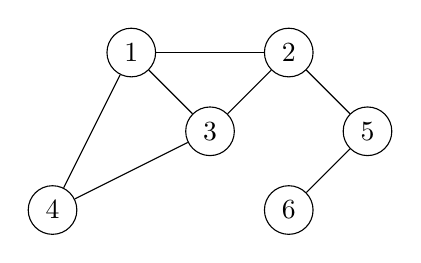
\begin{tikzpicture}
        \node[circle, draw] (1) at (0, 0) {1};
        \node[circle, draw] (2) at (2, 0) {2};
        \node[circle, draw] (3) at (1, -1) {3};
        \node[circle, draw] (4) at (-1, -2) {4};
        \node[circle, draw] (5) at (3, -1) {5};
        \node[circle, draw] (6) at (2, -2) {6};
        \draw[] (1) -- (2);
        \draw[] (1) -- (3);
        \draw[] (1) -- (4);
        \draw[] (2) -- (3);
        \draw[] (2) -- (5);
        \draw[] (3) -- (4);
        \draw[] (5) -- (6);
    \end{tikzpicture}
    
    \caption{A graph-theoretic example of a metric space. Let $X = \set{1, 2, 3, 4, 5, 6}$. Then, for $x, y \in X$, let $d(x, y)$ be the number of edges if the shortest path between $x$ and $y$. Properties (a), (b) of a metric are immediately satisfied, and (c) follows from the property of the shortest path.}
    \label{fig5}
\end{figure}


\setcounter{rudin}{17}
\begin{definition}{Neighbourhoods}{2.18a}
    A \textbf{neighbourhood} in a metric space $X$ is a set $N_r(p) = \set{q \in X: d(p, q) < r}$ with $r > 0$. 
\end{definition}

\begin{nexample}{}
    \begin{itemize}
        \item In $\RR$, $N_r(p)$ is the interval $(p - r, p + r)$ about midpoint $p$.
        \item In $\RR^2$, $N_r(p)$ is the open disk about center $p$. 
        \item In $\RR^3$, $N_r(p)$ is the open ball about center $p$.
        \item In $\RR^n$, $N_r(p)$ is the open hyperball about center $p$. 
    \end{itemize}
\end{nexample}
\setcounter{rudin}{17}

\begin{definition}{Interior Points}{2.18e}
    Let $E \subseteq X$. Then, $p$ is an \textbf{interior point} of $S$ if there is a neighbourhood $N_r(p)$ such that $N \subseteq E$. 
\end{definition}
\noindent Intuitively, an interior point of $E$ is a point that is not on the boundary of $E$. As an example, in $\RR^n$, if $E = \set{y: \abs{x - y} \leq 1}$, then the interior points of $E$ (which we can denote as $E^\circ$) are $E^\circ = \set{y: \abs{x - y} < 1}$. The idea is that there is always some finite distance to the boundary, so we can always fit a (perhaps small) open ball in. But this doesn't hold at the boundary!
\begin{figure}[htbp]
    \centering
    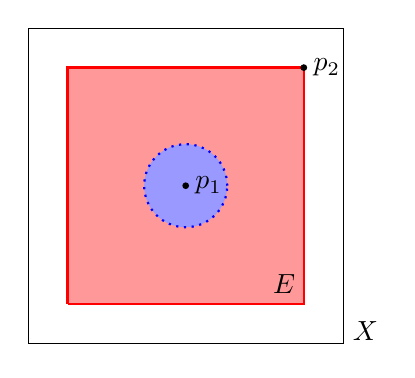
\begin{tikzpicture}
        \draw[] (-2, -2) -- (-2, 2) -- (2 ,2) -- (2, -2) -- (-2, -2);
        \draw[red, thick, fill = white!60!red] (-1.5, -1.5) -- (-1.5, 1.5) -- (1.5, 1.5) -- (1.5, -1.5) -- (-1.5, -1.5);
        \draw[blue, dotted, thick, fill = white!60!blue] (0, 0) circle (15pt);
        \draw[fill] (1.5, 1.5) circle (1pt);
        \draw[fill] (0, 0) circle (1pt);
        \node[right] at (0, 0) {$p_1$};
        \node[right] at (1.5, 1.5) {$p_2$};
        \node[] at (1.25, -1.25) {$E$};
        \node[right] at (2, -1.85) {$X$};
    \end{tikzpicture}
    \caption{A visualation of an interior point. A set $E \subset X$ is pictured. $p_1$ is an interior point as there exists $N_r(p_1) \subset E$. $p_2$ is not an interior point as there does not exist a neighbourhood of $p_2$ that is entirely contained in $E$ (it is on the boundary). }
    \label{fig6}
\end{figure}

\setcounter{rudin}{17}
\begin{definition}{Open Sets}{2.18f}
    A set $E \subseteq X$ is \textbf{open} if every point of $E$ is an interior point of $E$. 
\end{definition}

\begin{theorem}{}{2.19}
    Every neighbourhood is an open set.
\end{theorem}
\begin{nproof}
    Consider a neighbourhood $E = N_r(p) \subseteq X$. Let $q \in E$. We will show that $q$ is an interior point of $E$. Choose $s < r - d(p, q)$. Then, let $x \in N_s(q)$. By the triangle inequality:
    \begin{align*}
        d(x, p) \leq d(x, q) + d(q, p) < s + d(q, p) < r - d(p, q) + d(p, q) = r.
    \end{align*}
    Hence, $d(x, p) < r$ and it follows that $x \in N_r(p)$. Hence, $N_s(q) \subset N_r(p)$ and $q$ is an interior point of $E$. \qed
\end{nproof}

\begin{figure}[htbp]
    \centering
    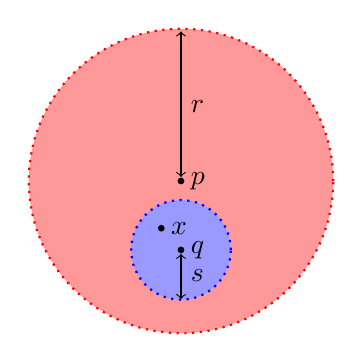
\begin{tikzpicture}
        \draw[red, dotted, thick, fill = white!60!red] (0, 0) circle (55pt);
        \draw[fill] (0, 0) circle (1pt);
        \node[right] at (0, 0) {$p$};
        \node[right] at (0, 0.95) {$r$};
        \draw[<->] (0, 0.05) -- (0, 1.9);
        \draw[blue, dotted, thick, fill = white!60!blue] (0, -0.875) circle (18pt);
        \draw[fill] (0, -0.875) circle (1pt);
        \node[right] at (0, -0.875) {$q$};
        \draw[<->] (0,-0.925) -- (0, -1.5);
        \node[right] at (0, -1.2) {$s$};
        \draw[fill] (-0.25, -0.6) circle (1pt);
        \node[right] at (-0.25, -0.6) {$x$};
    \end{tikzpicture}
    %\node[right] at (1.9, 0) {$N_r(p)$};
    %\node[right] at (0.6, -0.875) {$N_s(q)$};
    \caption{Visualization of the Sets/Points in Theorem \ref{thm:2.19}}
    \label{fig7}
\end{figure}

\setcounter{rudin}{17}
\begin{definition}{Limit Points/Isolated Points}{2.18b}
    Let $E \subseteq X$ and $p \in X$. Then, $p$ is a \textbf{limit point} of $E$ if every neighbourhood of $p$ contains $q \in E$, $q \neq p$. If $p \in E$ and $p$ is not a limit point of $E$, then $p$ is an \textbf{isolated point} of $E$. 
\end{definition}
\begin{nexample}{}{}
    Let $E = \set{\frac{1}{n}: n \in \NN}$. Then, $\frac{1}{2}$ is not a limit point of $E$, as for $r < \frac{1}{4}$ $N_r(\frac{1}{2})$ does not contain any other points of $E$. On the other hand, $0$ is a limit point of $E$. For any neighbourhood $N_r(0)$ of $0$, $\frac{1}{N} \in N_r(0)$ for $N > \frac{1}{r}$. Note that $0$ is the only limit point of $E$, and is not contained in $E$ (indeed, there is no requirement that a limit point be contained in the set). 
\end{nexample}

\setcounter{rudin}{19}

\begin{theorem}{}{2.20}
    If $p$ is a limit point of $E$, then every neighbourhood of $p$ contains an infinite number of $q \in E$. 
\end{theorem}

\begin{nproof}
    (Sketch) Let $r_1 = 1$. Then, there exists $q_1 \in N_{r_1}(p)$ such that $q_1 \in E$ and $q_1 \neq p$ as $p$ is a limit point of $E$ by assumption. Let $r_2 = d(q_1, p)$. Then, there exists $q_2 \in N_{r_2}(p)$ such that $q_2 \in E$ and $q_2 \neq p$. We can repeat this process to get a (countably infinite) sequence of distinct points $q \in N_{r_1}(p)$, which proves the claim. \qed 
\end{nproof}

\begin{ncorollary}{}{}
    If $E \subseteq X$ is finite, then $E$ has no limit points.
\end{ncorollary}

\setcounter{rudin}{17}
\begin{definition}{Closed Sets}{2.18d}
    A set $E \subseteq X$ is closed if every limit point of $E$ is in $E$. 
\end{definition}
\noindent Note that with the above Corollary, we find that every finite set is (trivially) closed.

\setcounter{rudin}{17}
\begin{definition}{Complement}{2.18g}
    Let $E \subseteq X$. Then, the complement of $E$, denoted $E^c$ is $E^c = \set{x \in X: x \notin E}$. 
\end{definition}
\begin{figure}[htbp]
    \centering
    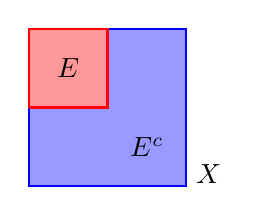
\begin{tikzpicture}
        \draw[] (-1, -1) -- (1, -1) -- (1, 1) -- (-1, 1) -- (-1, -1);
        \draw[blue, thick, fill = white!60!blue] (-1, 0) -- (-1, -1) -- (1, -1) -- (1, 1) -- (0, 1) -- (0, 0) -- (-1, 0);
        \draw[red, thick, fill = white!60!red] (-1, 0) -- (0, 0) -- (0, 1) -- (-1, 1) -- (-1, 0);
        \node at (-0.5, 0.5) {$E$};
        \node at (0.5, -0.5) {$E^c$};
        \node[right] at (1, -0.85) {$X$};
    \end{tikzpicture}
    
    \caption{Visualization of a set $E$ and its complement.}
    \label{fig8}
\end{figure}

\setcounter{rudin}{22}
\begin{theorem}{}{2.23}
    A set $E \subseteq X$ is open if and only if $E^c$ is closed.
\end{theorem}
\noindent Note that this theorem does not imply that all sets are closed or open; it is possible to have a set that is neither closed or open (such as $[0, 1) \subset \RR$) and then its complement (with the former example, $(-\infty, 0) \cup [1, \infty]$) which is also neither closed nor open. As an additional note, we have that $X$ (the entire metric space) and $\emptyset$ are both open and closed (which we may affectionately label as ``clopen'').

\begin{nproof}
    \boxed{\implies} Assume $E$ is open. If $E^c$ has no limit points, it is trivially closed, so suppose that there exists a limit point $x$ of $E^c$. Suppose for the sake of contradiction that $x \notin E^c$. Then, $x \in E$. As $E$ is open, $x$ is an interior point of $E$, so there exists a neighbourhood $N_r(x) \subseteq E$. In particular, $N_r(x) \cap E^c = \emptyset$, contradicting the fact that $x$ is a limit point of $E^c$. Hence, $x \in E^c$ and $E^c$ is closed.

    \boxed{\impliedby} Assume $E^c$ is closed. Let $x \in E$. In particular, $x \notin E^c$, so $x$ is not a limit point of $E^c$. So, there exists a neighbourhood $N_r(x)$ which contains no point of $E^c$, i.e. $N_r(x) \cap E^c = \emptyset$. It follows that $N_r(x) \subseteq E$, and hence $x$ is an interior point of $E$. This argument applies to all points of $E$, hence $E$ is open. \qed
\end{nproof}

\begin{ncorollary}{}{}
    A set $F \subseteq X$ is closed if and only if $F^c$ is open.
\end{ncorollary}
\noindent Let $F = E^c$ in Theorem \ref{thm:2.23} to realize the above Corollary.

\begin{theorem}{}{2.24}
    \begin{enumerate}
        \item For any collection $\set{E_\alpha}$ of open sets, $\bigcup_\alpha E_\alpha$ is open.
        \item For any collection $\set{F_\alpha}$ of closed sets, $\bigcap_\alpha F_\alpha$ is closed.
        \item For any finite collection $E_1, \ldots, E_n$ of open sets, $\bigcap_{i=1}^n E_i$ is open.
        \item For any finite collection $F_1, \ldots, F_n$ of closed sets, $\bigcup_{i=1}^n F_i$ is closed.
    \end{enumerate}
\end{theorem}
\noindent A point of notation; $\set{E_\alpha}$ can be finite, countable, or uncountable; the indices $\alpha$ are taken from an index set $A$ which can be chosen to be of any cardinality. 
\begin{nproof}
    \begin{enumerate}
        \item Suppose all sets in $\set{E_\alpha}$ are closed. Let $x \in \bigcup_{\alpha}E_\alpha$. Then, there exists $\alpha_0$ such that $x \in E_{\alpha_0}$. Since $E_{\alpha_0}$ is open, there exists a neighbourhood $N_r(x)$ of $x$ such that $N_r(x) \subseteq E_{\alpha_0} \subseteq \bigcup_{\alpha} E_\alpha$. Hence, $\bigcup_{\alpha} E_\alpha$ is open.
        \item Suppose all sets in $\set{F_\alpha}$ are open. To show that $\bigcap_\alpha F_\alpha$ is closed, we show that $\left(\bigcap_\alpha F_\alpha\right)^c$ is open (by Theorem \ref{thm:2.23}). We have that $\left(\bigcap_\alpha F_\alpha\right)^c = \bigcup_\alpha F_\alpha^c$. As all $F_\alpha^c$ are open, by part (a) we have that $\bigcup_\alpha F_\alpha^c$ is also open. Hence $\bigcap_\alpha F_\alpha$ is closed.
        \item Suppose $E_1,\ldots, E_n$ are open. Let $x \in \bigcap_{i=1}^n E_i$, and then we have that $x \in E_i$ for all $i \in \set{1, \ldots, n}$. Hence, there exists $r_i$ such that $N_{r_i}(x) \subseteq E_i$ as each of the $E_i$s are open. Let $r = \min\set{r_1, \ldots, r_n}$ and then we have that $N_r(x) \subseteq N_{r_i}(x) \subseteq E_i$ for all $E_i$. Therefore, $N_r(x) \subseteq \bigcap_{i=1}^n E_i$ and $\bigcap_{i=1}^n E_i$ is open.
        \item Suppose $F_1, \ldots, F_n$ are closed. By Theorem \ref{thm:2.23} we have that $\bigcup_{i=1}^n F_i$ is closed if and only if $\left(\bigcup_{i=1}^n F_i\right)^c = \bigcap_{i=1}^n F_i^c$ is open. Since all $F_i^c$s are open, by part (c) $\bigcap_{i=1}^n F_i^c$ is open, and hence $\bigcup_{i=1}^n F_i$ is closed. \qed
    \end{enumerate}
\end{nproof}

\begin{example}{}{2.25}
    We consider some examples to see why the finiteness of the collections in parts (c)/(d) of the theorem are essential. Suppose $E_n = \left(-\frac{1}{n}, \frac{1}{n}\right) \subset \RR$. These sets form a countably infinite collection of subsets of $\RR$. We then consider that $\bigcap_{n=1}^\infty E_n = \set{0}$, which is not open; showing that openness is not preserved under infinite intersections. Next, consider $F_n = [0, 1-\frac{1}{n}] \subset \RR$, which form a countably infinite collection of closed sets in $\RR$. We then have that $\bigcup_{n=1}^\infty F_n = [0, 1)$ which is not closed as $0$ is not an interior point of the set. Hence, closedness is not preserved under infinite unions. 
\end{example}

\subsection{Closure and Relative Topology}
\subsection{Compactness}
\subsection{Compactness in \texorpdfstring{$\RR^k$}{TEXT} and the Cantor Set}
